\chapter{背景}

\section{GC}
GC(垃圾收集)是托管式语言Java、Scala等与非托管式语言像C或C++的主要区别之一。
使用托管式语言进行开发,不需要专门编写内存分配与回收代码,也不需要去考虑
内存泄漏和溢出的问题。这确实给开发人员降低了不少工作压力,但也带来了两个新问题。
其一,GC时间开销太大,成为性能瓶颈,降低可扩展性。其二,由于内存管理都是托管的,
开发人员不能详细了解内存管理情况。这就导致一旦发生内存溢出与内存泄漏问题,开发人员
需要花更多的精力去解决。换言之,由于内存管理是托管的,内存管理的正确性与性能也都由
托管式语言对应的高级语言虚拟机(Java语言的JVM,.Net语言的CLR等)决定。所以一旦虚拟机的
垃圾回收策略与当前运行场景不适配(这常常发生,因为虚拟机的垃圾回收策略相对稳定,
大约2-3年才会更新一次,但是新场景层出不穷,所以往往策略是不能完全适配场景),那么内存管理的性能与正确性都会变得很糟糕。
GC的任务是解决以下三个问题:哪些内存需要回收、什么时候回收和如何回收。

\begin{figure}[h]
    \centering
    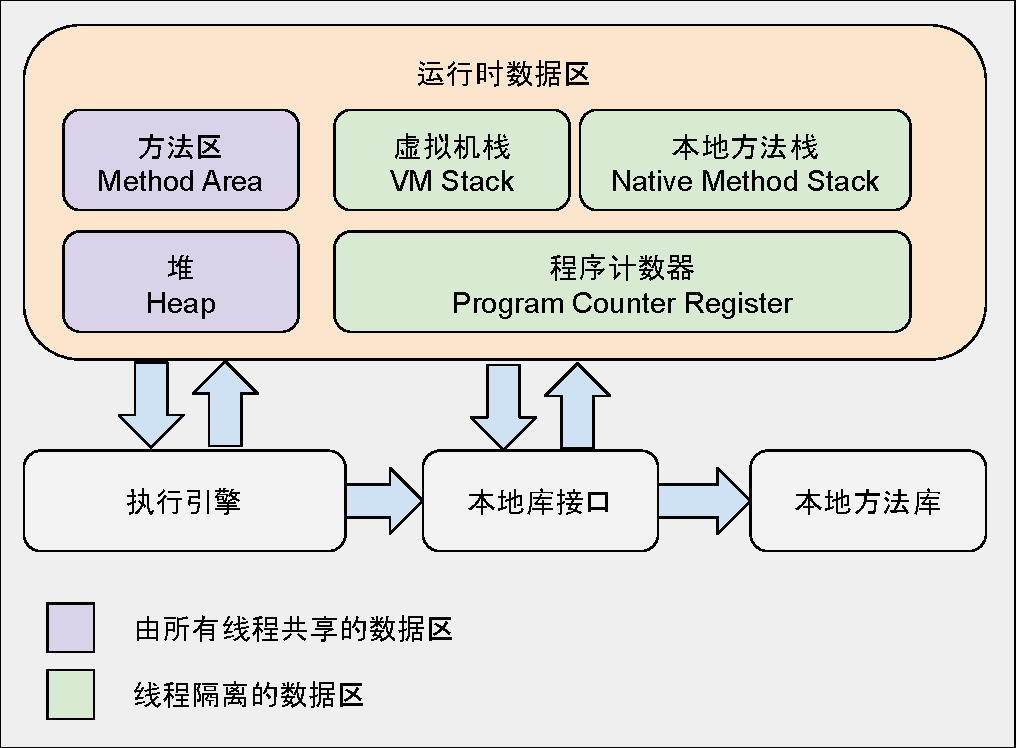
\includegraphics[width=12cm]{figure/JVM_memory_layout.pdf}
    \caption{JVM运行时数据区\cite{Understand_JVM}}
    \label{jvm_memory_layout}
\end{figure}

回答这三个问题首先需要了解虚拟机中的内存布局。以JVM为例,JVM在执行Java程序的过程中会把他所管理的内存划分为弱冠个不同的数据区域。
JVM运行时数据区如图\ref{jvm_memory_layout}所示。程序计数器存储正在执行的虚拟机字节码的地址。虚拟机栈包含局部变量表、操作数栈、动态链接、方法出口等信息。
其中局部变量表所需的内存空间在编译时完成分配,当进入一个方法时,这个方法需要在帧中分配多大的局部空间是完全确定的,不会改。
本地方法栈存储JNI调用。堆在虚拟机启动时创建,此内存区域唯一目的是存放对象实例。所有的对象实例和数据都要在堆上分配,
但是随着JIT编译器的发展与逃逸分析技术逐渐成熟,栈上替换、标量替换将会导致一些微妙的变化。方法区
存储被虚拟机加载的类信息、常量、静态变量、即时编译器编译后的代码等数据。其中方法区和堆是线程共享的,
也是JVM GC所针对的数据区。

哪些内存需要回收?托管式语言虚拟机中,数据是以对象的形式存储在堆中,对象由对象头、实例数据和对齐三部分组成。
其中对象头包含对象自身运行时的数据包括对象的hashcode、GC分代年龄等;实例数据包含对象的属性数据包括以指针形式存在的
指向其他对象的引用。GC主要针对的是堆中未被引用的对象。寻找未被引用对象是通过可达性分析算法实现的。可达性分析算法以
\texttt{GC Root}对象作为起点沿着对象间的引用链向下搜索,搜索不到的对象为不可达对象,GC时会被回收。\texttt{GC Root}
是GC被调用时一定存活的对象,JVM中\texttt{GC Root}由以下四种对象组成:
\begin{enumerate}
    \item 虚拟机栈(栈帧中的本地变量表)中引用的对象
    \item 方法区中类静态属性引用的对象
    \item 方法区中常量引用的对象
    \item 本地方法栈中JNI引用的对象
\end{enumerate}

在内存不够用时,虚拟机会调用GC。那么GC是如何运行的?虚拟机是通过不同的垃圾收集算法来执行GC的。包括标记-清除算法、
标记-整理算法、复制算法、分代收集算法和基于region的分代收集算法。标记-清除算法是指通过可达性分析标记出不可达对象后,直接清除。
标记-清除算法有两个不足:其一,清除之后会产生大量碎片,无法分配大对象;其二标记与清除两个过程都是针对整个堆,比较耗时。
复制算法将可用内存分为大小相等的两块,每次只使用其中一块,当一块内存用完时,将这块内存上还存活的对象复制到另一块内存上去,再将这一块内存全部清理掉。
复制算法解决了大量数据对象需要被清除时,清理耗时的问题,提高了效率,也解决了碎片化的问题。但是可用内存减小了,并且如果存活对象较多,复制也会比较耗时。
标记-整理算法将存活对象向顶端或低端移动,清除边界之外的对象,解决了标记-清除算法的碎片化问题,也较为高效,并且相对于复制算法,
标记-整理算法使用了全部的内存。

标记-清除算法、标记-整理算法和复制算法都是对整个堆进行标记和移动,当对象分配的越来越多时,标记和移动也越来越耗时。
但是,根据对Java应用的分析,数据对象的生命周期是不一样的。大部分对象的生命周期很短,小部分对象的生命周期很长。
分代收集算法就是基于这种观察结果被提出的。
分代收集算法将数据对象根据生命周期的不同分为新生代和老生代,并且将堆空间分为几块用来存放不同生命周期的对象,
分别应用最合适的垃圾收集算法。新生代生命周期较短,GC过后只有少量存活,所以使用复制算法。老生到对象存活率较高,
使用标记-清除或者标记-整理算法。对象被创建时,大对象直接进入老生代,小对象就在新生代进行分配,多次GC后任然
存活的对象会进入老生代。一般老生代会占据60\%以上的堆空间。显然新生代相较于老生代GC会比较频繁,新生代GC也只要对
新生代的做可达性分析,然后使用复制算法,老生代GC次数较少。因此分代收集算法提供了最高的收集效率。

\begin{figure}[h]
    \centering
    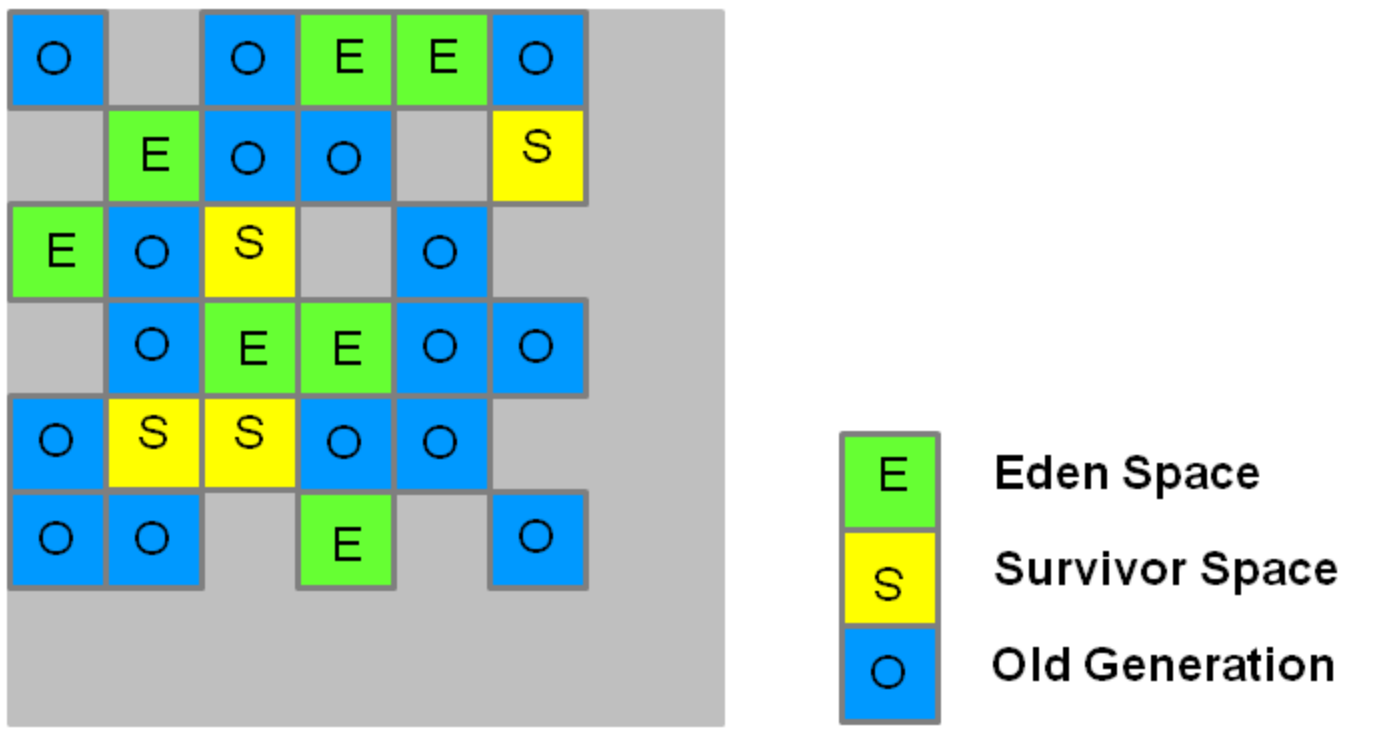
\includegraphics[width=12cm]{figure/region-based-gc.png}
    \caption{基于region的分代收集算法堆空间布局\cite{G1}}
    \label{jvm_region-gc}
\end{figure}
在相同条件下, 堆空间越大, 一次GC耗时就越长, 从而产生的停顿也越长。分代收集算法将堆空间划分为新生代与老生代两部分,
相较于之前,极大提高了效率。但是GC开销还是过大,现代服务器要求每次GC的时间要尽量短,最好控制在某个上限之下。因此
基于region的分代收集算法(又名分区分代收集算法)应运而生。如图\ref{jvm_region-gc}为了更好地控制GC产生的停顿时间, 基于region的分代收集算法将一块大的内存区域分割为多个小块, 
根据目标停顿时间, 每次合理地回收若干个小区间(而不是整个堆), 从而减少一次GC所产生的停顿。基于region的分代收集算法是目前
最新的垃圾收集算法,其性能也最忧。

大数据场景中,数据对象可以按控制路径与数据路径分为用于分布式节点调度的对象和用于装载数据、计算并表示结果的对象。
控制路径对象的生命周期符合新生代老生代的分代特征,使用分代收集算法即可。但是数据路径对象生命周期不符合分代特征。
它们的生命周期呈现出与完全不同的epoch特性,不适合传统GC。epoch特性是指一组对象在同一时间被创建,
在经历一段较长的程序执行时间后可以同时被回收。因此,大数据场景下,传统GC不适配,往往带来巨大的性能开销。

